\chapter{Summary of Gulwani and Necula}
\label{chap:chapter3}

Gulwani showed that there is a family of acyclic programs for which 
the set of all Herbrand equivalences requires requires an exponential 
sized (with respect to the size of the program) value graph 
representation - the data structure used by Kildall in his algorithm. 
He also showed that Herbrand Equivalences among program sub 
expressions can always be represented using linear sized value graph. 
This explains the reason for exponential complexity of Kildall's 
algorithm which cannot be improved to polynomial and imprecise nature 
of existing polynomial time algorithms.

So contrasting to Kildall's algorithm, which finds \textit{all the 
Herbrand Equivalent classes} corresponding to constants, variables 
and operators occurring in the program, Gulwani's algorithm discovers 
\textit{equivalences among program subexpressions} (expressions that 
can occur syntactically in a program), in linear time with respect to 
parameter $s$, the maximum size of an expression in terms of number 
of operators used. For global value numbering, $s$ can be safely 
taken to be $N$, the size of the program and hence the algorithm is 
linear in the program size.

Also, he proved that the lattice of sets of Herbrand equivalences has 
finite height $k$, which is the number of program variables. So, an 
abstract interpretation over the lattice of Herbrand equivalences 
will terminate in at most $k$ iterations even for cyclic programs.

\section{Brief overview of the algorithm}
The program expressions considered can be represented as
$$e\; ::=\; x\: |\: c\: |\:F(e_1, e_2)$$
Here, $c$ and $x$ are constants and variables occurring in the 
program.

The data structure used is called \textit{Strong Equivalence DAG 
(SED)}. Each node is of the form $<V,t>$ where $V$ is a set of 
program variables and $t$ is either $\perp$ or $c$ for leaf nodes and 
$F(n_1, n_2)$ where $n_1$ and $n_2$ are SED nodes for non leaf nodes
(also indicating that the node has two ordered successors). $\perp$ 
means that the variables in the node have undefined values.

There is a SED associated with each program point and the algorithm
starts with the following initial SED
$$G_0\; =\; \{<x,\perp>\: |\: x \text{ is a program variable}\}$$ 
Two functions $Join(G_1, G_2, s')$ and $Assignment(G_1, x := e)$ are 
used to compute SEDs for other points in the flow graph node 
corresponding to the program, as shown in figure 
\ref{fig:GulwaniAlgorithm}. $s'$ in the argument of \textit{Join} is 
a positive integer, and it returns equivalences between expressions of
size atmost $s'$.

\begin{figure}[!h]
    \centering {
        \setlength{\fboxsep}{8pt}    
        \fbox{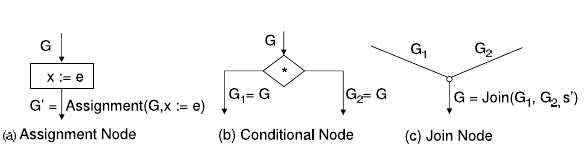
\includegraphics[scale=0.5]{GulwaniAlgorithm.png}}
    }
    \caption{Computation of SED for flowgraph nodes of a program}
    \label{fig:GulwaniAlgorithm}
\end{figure}

For detailed implementation of \textit{Join} and \textit{Assignment} 
and correctness proof of the algorithm, see \cite{Gulwani}.

\section{Complexity of the algorithm}
The complexity of the algorithm is $O(k^{3} * N * j)$, where $k$ is  
the total number of program variables, $N$ is the size of the program 
and $j$ is the number of join operations in the program. $k$ and $j$ 
are bounded by $N$, making the whole algorithm polynomial in $N$.